\documentclass[conference]{IEEEtran}
\IEEEoverridecommandlockouts
% The preceding line is only needed to identify funding in the first footnote. If that is unneeded, please comment it out.
\usepackage{cite}
\usepackage{amsmath,amssymb,amsfonts, amsthm}
\usepackage{algorithmic}
\usepackage{graphicx}
\usepackage{textcomp}
\usepackage{xcolor}
\usepackage{epstopdf}
\graphicspath{{../Figures/}}
%\def\BibTeX{{\rm B\kern-.05em{\sc i\kern-.025em b}\kern-.08em
%    T\kern-.1667em\lower.7ex\hbox{E}\kern-.125emX}}
\newtheorem{prop}{Proposition}
\newtheorem{defi}{Definition}
\newtheorem{theo}{Theorem}
\newtheorem{lem}{Lemma}
\newtheorem{clm}{Claim}
\newtheorem{coro}{Corollary}
\begin{document}

\title{Finite Blocklength Rates over a Fading Channel with an Energy Harvesting Transmitter\\
%{\footnotesize \textsuperscript{*}Note: Sub-titles are not captured in Xplore and
%should not be used}
%\thanks{Identify applicable funding agency here. If none, delete this.}
}

\author{\IEEEauthorblockN{Void Ship}
\IEEEauthorblockA{\textit{Dept. of ECE} \\
\textit{Indian Institute of Science}\\
Bangalore, India \\
voidship@IISc.ac.in}
\and
\IEEEauthorblockN{$D(P||K)$}
\IEEEauthorblockA{\textit{Dept. of ECE} \\
\textit{Indian Institute of Science}\\
Bangalore, India \\
d(p$||$k)@IISc.ac.in}
\and
\IEEEauthorblockN{Vinod Sharma}
\IEEEauthorblockA{\textit{Dept. of ECE} \\
\textit{Indian Institute of Science}\\
Bangalore, India \\
vinod@IISc.ac.in}
}

\maketitle

\begin{abstract}
This document is a model and instructions for \LaTeX.
This and the IEEEtran.cls file define the components of your paper [title, text, heads, etc.]. *CRITICAL: Do Not Use Symbols, Special Characters, Footnotes, 
or Math in Paper Title or Abstract.
\end{abstract}

\begin{IEEEkeywords}
component, formatting, style, styling, insert
\end{IEEEkeywords}

\section{Introduction}
Finite blocklength analysis for channels with fading under various power control schemes is available in \cite{deeks2018}.

\subsection{Main Contributions}
\section{Model and Notation}
Consider a wireless communication system powered by an energy harvesting transmitter, as depicted in Figure \ref{Fig_Schematic}. The energy harvesting system consists of an energy buffer or battery that provides power to transmit symbols. The buffer harvests energy $E_i\geq 0$ at time instant $i$ from the ambient environment. We assume these energy arrivals are independent and identically distributed (i.i.d.) with mean $\overline{E}$ and variance $\sigma_E^2$. Further details on the transmitter are discussed in Section \ref{Txmod}.

The transmitter selects a message $S$ uniformly randomly from the set $[1:M]$ (in general, we denote the set of $j$ consecutive natural numbers starting from $\ell$  as $[\ell:\ell+j-1]$). The encoder maps this message to an $n$ length codeword $\mathbf{X}'\triangleq \left(X_{1}',X_{2}',\dots, X_{n}'\right)$, where $X_{i}'\in\mathbb{C}$ (the set of complex numbers) for $i\in[1:n]$. This codeword is to be transmitted across a wireless channel and hence some processing may be carried out (in order to meet channel constraints etc.) on $X_i'$. Therefore, let $X_i$ denote the corresponding input to the channel after processing. Next, we describe our channel model. 

\subsection{Channel Model}
Let $\tau_c$ (in appropriate time units) denote the coherence time of the underlying wireless channel. We refer to any \emph{coherence period} of duration $\tau_c$ as a \emph{block}. Let $D$ denote the maximum delay permissible at the physical layer (as dictated by the application). For convenience, assume that $D$ is an integer multiple of $\tau_c$. Then, $B\triangleq D/\tau_c$ denotes the number of blocks over which the communication happens.   Let $n_c$ denote the number channel uses in each block. We consider a discrete time block fading channel in which the fading gain $H_b\in\mathbb{C}$ in block $b\in[1:B]$ remains constant for all $n_c$ uses within the block. The fading gains are independently and identically distributed (i.i.d.) across blocks.  Let $F_{H}$ (assumed to be known to both the transmitter and the receiver) denote the cumulative distribution distribution of $H_b$, $b\in[1:B]$. We assume $F_{H}$ is such that $\int_{\mathbb{C}}|h|^2dF_H(h)\equiv \sigma_H^2<\infty$, where $|h|$ denotes the absolute value of the complex number $h$. 
\par For $k\in[1:n_c]$, $k$\textsuperscript{th} transmission in $b$\textsuperscript{th} block corresponds to the transmission of $\left((b-1)n_c+k\right)$\textsuperscript{th} codeword symbol. For convenience, let $[b, k]\triangleq (b-1)n_c+k$. Note that $[b, 0] = [b-1, n_c]$ and $[b, n_c+1] = [b+1, 1]$. Then, the additive receiver noise corresponding   to $k$\textsuperscript{th} transmission in $b$\textsuperscript{th} block is denoted as $Z_{[b,k]}$. We assume that $\left\{Z_{[b,k]},k\in[1:n_c],b\in[1:B]\right\}$ is independent and identically distributed according to $\mathcal{C}\mathcal{N}\left(0,\sigma_N^2\right)$, where $\mathcal{C}\mathcal{N}\left(0,\sigma_N^2\right)$ the probability density function of a circularly symmetric, complex Gaussian random variable  with mean vector $[0,0]$ and covariance matrix $\frac{\sigma_N^2}{2}I_2$ with $I_2$ being the $2\times 2$ identity matrix.

\subsection{Transmitter Model}\label{Txmod}
We assume that the transmitter is equipped with a battery (equivalently, a buffer or a \emph{cell}) with infinite storage capacity. Let $A_{[b,k]}$ correspond to the energy available in the cell at the beginning of $k$ \textsuperscript{th} transmission in $b$\textsuperscript{th} block. Let $E_{[b,k]}$ denote the energy harvested at the beginning of $k$\textsuperscript{th} transmission in $b$\textsuperscript{th} block. We assume that the total energy available at the beginning of $k$\textsuperscript{th} transmission in $b$\textsuperscript{th} block is $E_{[b,k]}+A_{[b,k]}$ and that the energy buffer is initially empty i.e. $E_0 = 0$. 
\begin{figure}[h]
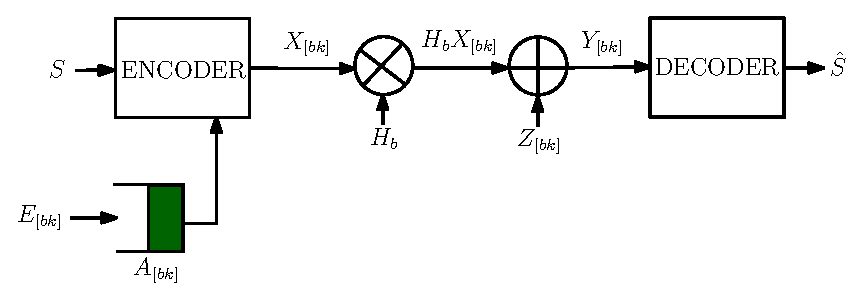
\includegraphics[scale=.6]{Schematic_BlockFade_EHTx.eps}
\caption{Block diagram of a wireless communication system with energy harvesting transmitter}
\label{Fig_Schematic}
\end{figure}

The buffer state $A_{[b,k]}$ evolves according to the equation
\begin{equation}
	A_{[b,k+1]} = \max\{A_{[b,k]} + E_{[b,k+1]} - X^2_{[b,k+1]}, 0 \},
\end{equation}
since the buffer cannot be negative. If at any instant the symbol to be transmitted requires more energy than what is available (including harvested energy), we refer to it as an energy outage event. It is worth observing that if there was sufficient energy to transmit every symbol (for a given input distribution), then it would be equivalent to studying the channel alone for that input. Unfortunately this is an unlikely event for several useful distributions (including capacity achieving distributions) and hence, a suitable transmission scheme or policy is required. Two well known and studied schemes are the Save and Transmit scheme as well as the Best Effort scheme. In this paper, we focus on the former as it is known to provide the optimal second order term (not necessarily the coefficient). 

\subsection{Save and Transmit Scheme}
This scheme consists of two phases, namely the saving phase and the transmission phase. During the saving phase, no symbols are transmitted and the energy buffer is allowed to build up. During the transmission phase, we start transmitting symbols but now, the buffer contains some energy. This initial energy helps to lower, and hence control, the probability of energy outage. The tradeoff here is the number of slots where we don't transmit anything which is, as far as information transfer is concerned, wasted. However by carefully choosing the duration, we can achieve a balance of sorts.

\subsection{Known Results and Useful Lemmas}
We recall known finite blocklength bounds for energy harvesting AWGN channels \cite{mycon1, Tan1, TanF2} as well as the fading channel with \emph{long term} power constraint \cite{deeks2018, polyf}. 

\begin{lem}\label{Lem1}
		Consider a EH-AWGN channel, with AWGN variance $\sigma^2$, with energy harvesting process $\{E_i\}$, i.i.d. at the encoder, with mean $\mathbb{E}[E_1]$ and variance $\sigma_E^2 < \infty$. 
		\begin{enumerate}
			\item (Achievable bound) Given maximal probability of error $\varepsilon>0$ and any $0 < \lambda < 1$, for sufficiently large blocklength $n$, the maximum size of the code, $M^*(n,\varepsilon)$, is lower bounded by 
			\begin{IEEEeqnarray}{rCl}
			\log M^*(n, \varepsilon) &\geq& nC_{EG}+ \sqrt{n}\left[\sqrt{V_{EG}}\Phi^{-1}\left(\lambda\varepsilon\right)\right.\notag \\
			&& \left.-K_{\varepsilon, \lambda}C_{EG}\right]-\frac{1}{2}\log n + O(1),
			\label{ehawgnclb}
			\end{IEEEeqnarray}
			where $V_{EG} = \frac{\mathbb{E}[E_1]}{\mathbb{E}[E_1] + \sigma^2}\log^2_2(e)$, $K_{\varepsilon, \lambda} = \sqrt{\frac{4(2\mathbb{E}[E_1]^2 + \sigma_E^2 )}{(1-\lambda) \varepsilon \mathbb{E}[E_1]^2}}$.
			
			\item (Converse Bound) The upper bound on $M^*(n,\varepsilon)$ is given by
			\begin{equation}
			\log M^*(n, \varepsilon) \leq nC_{EG} +\sqrt{nV_{EG2}}\Phi^{-1}(\varepsilon) + \frac{1}{2}\log n +O(1)
			\label{ehawgncub}
			\end{equation}
			where $V_{EG2} = \frac{\mathbb{E}[E_1]^2 + \mathbb{E}[E_1^2] + 4\sigma^2\mathbb{E}[E_1]}{4(\mathbb{E}[E_1]+\sigma^2)^2}\log_2^2(e)$.
		\end{enumerate}
\end{lem}
Putting it concisely, $\log M^*(n,\varepsilon) = nC + \Theta(\sqrt{n})$.
\bibliographystyle{IEEEtran}
\bibliography{EHFade}

\end{document}
